%This is a experiment example of ZhengXiaoyang's experiment report template

\documentclass[UTF8]{ctexart}

\usepackage{pythonhighlight}
\usepackage{amsmath}
\usepackage{cases}
\usepackage{cite}
\usepackage{xeCJK}
\usepackage{graphicx}
\usepackage[margin=1in]{geometry}
\geometry{a4paper}
\usepackage{fancyhdr}
\pagestyle{fancy}
\fancyhf{}

\graphicspath{{picture/}}


\title{RLC稳态电路实验报告}
\graphicspath{{picture/}}


\title{RLC稳态电路实验报告}
\author{郑晓旸}
\date{\today}
\pagenumbering{arabic}

\begin{document}
%这里是文件的开头
\fancyhead[L]{郑晓旸}
\fancyhead[C]{RLC稳态}
\fancyfoot[C]{\thepage}

\maketitle
\tableofcontents
\newpage

\section{实验目的}
    \begin{enumerate}
            \item 了解电感和电容的电学特性 
            \item 深入理解 RLC 串联谐振电路的特性
            \item 掌握用示波器观察和测量稳态信号的方法
    \end{enumerate} 



\section{实验仪器}
\begin{enumerate}
    \item 数字示波器
    \item 信号发生器
    \item 九孔电路实验板
    \item 电学元件(电阻、电容、电感、导线等)
    \item 数字多用表
\end{enumerate}


\section{实验原理}

\subsection{电感器和电容器}

电感器和电容器是常见的无源电路元件。理想电感器的伏安特性为:
\begin{equation}
u(t) = L\frac{di(t)}{dt}
\end{equation}
其中,$u(t)$为电感两端电压,$i(t)$为通过电感的电流,$L$为电感值,单位为亨利(H)。

理想电容器的伏安特性为:
\begin{equation}
i(t) = C\frac{du(t)}{dt}
\end{equation}
其中,$i(t)$为流经电容的电流,$u(t)$为电容两端电压,$C$为电容值,单位为法拉(F)。

\subsection{RLC串联谐振电路}

如图\ref{fig:rlc_circuit}所示,RLC串联谐振电路由电阻$R$、电感$L$和电容$C$串联而成,交流电压源为$u(t)=u_0\sin(\omega t)$。
\begin{figure}[htbp]
\centering
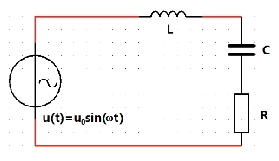
\includegraphics[width=0.6\textwidth]{rlc_circuit.png}
\caption{RLC串联谐振电路}\label{fig:rlc_circuit}
\end{figure}

根据基尔霍夫电压定律,电路方程为:
\begin{equation}
L\frac{d^2u_C(t)}{dt^2} + R\frac{du_C(t)}{dt} + \frac{1}{C}u_C(t) = u_0\sin(\omega t)
\end{equation}
其中,$u_C(t)$为电容两端电压。引入固有频率$\omega_0$和品质因数$Q$:
\begin{equation}
\omega_0 = \frac{1}{\sqrt{LC}}, \quad Q = \frac{1}{R}\sqrt{\frac{L}{C}}
\end{equation}
电路方程可改写为:
\begin{equation}
\frac{1}{\omega_0^2}\frac{d^2u_C(t)}{dt^2} + \frac{1}{Q\omega_0}\frac{du_C(t)}{dt} + u_C(t) = u_0\sin(\omega t)
\end{equation}

该方程的稳态解为:
\begin{equation}
\begin{cases}
\frac{u_C(t)}{u_0} = -\frac{Q\omega_0}{\omega}A\cos(\omega t + \phi) \\
\frac{u_R(t)}{u_0} = A\sin(\omega t + \phi) \\
\frac{u_L(t)}{u_0} = \frac{Q\omega}{\omega_0}A\cos(\omega t + \phi)
\end{cases}
\end{equation}
其中,
\begin{equation}
A = \frac{1}{\sqrt{1 + Q^2(\frac{\omega_0}{\omega} - \frac{\omega}{\omega_0})^2}}, \quad
\phi = \arctan\left[Q\left(\frac{\omega_0}{\omega} - \frac{\omega}{\omega_0}\right)\right]
\end{equation}

$A(\omega)$和$\phi(\omega)$分别称为电路的幅频特性和相频特性,统称为频率特性。当$\omega=\omega_0$时,电路达到谐振状态,此时$A(\omega_0)=1$,$\phi(\omega_0)=0$。品质因数$Q$反映了谐振时的电压放大倍数、频率选择性以及能量耗散的快慢。

\subsection{实验过程和数据分析}
本实验使用九孔板搭建RLC串联谐振电路,并通过示波器观察电压波形,测量电压幅值和相位差。实验过程如下:
\subsubsection{搭建RLC电路}
按图\ref{fig:rlc_circuit}搭建RLC串联谐振电路,其中电路元件参数如下表。
\begin{table}[htbp]
\centering
\caption{电路元件参数}
\begin{tabular}{lllll}
\hline
元件&特征值&单位&电阻值&单位\\
\hline
电感&10&mH&14.25&Ohm\\
\hline
电阻&1000&Ohm&990&Ohm\\
\hline
电容&1&uf&N/A&N/A\\
\hline
\end{tabular}
\end{table}

接入交流信号源,在输入和电阻两端接入示波器并保证两者共地,观察电压波形。搭建电路实物图如下:
\newpage
\begin{figure}[htbp]
\centering
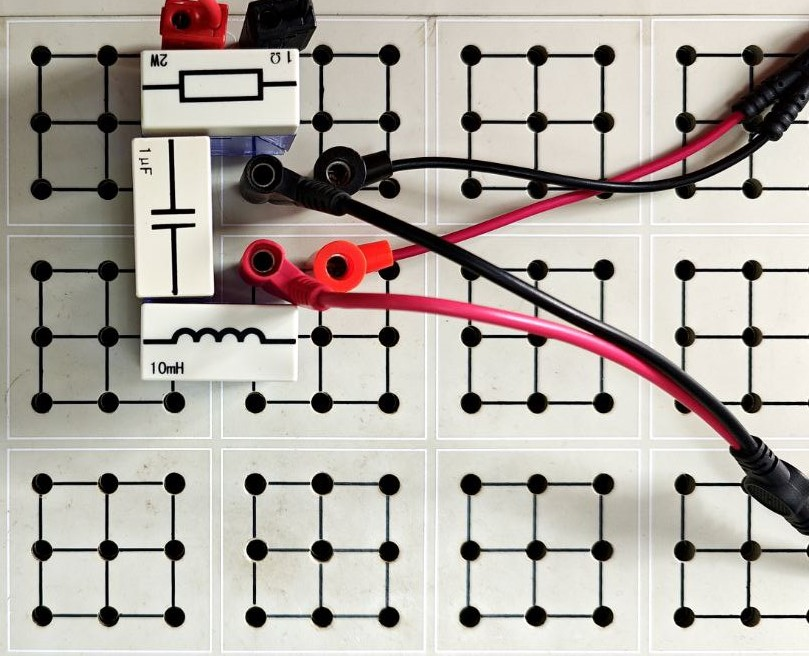
\includegraphics[width=0.6\textwidth]{circuit.jpg}
\caption{RLC串联谐振电路实物图}\label{fig:circuit}
\end{figure}
\subsubsection{调整输入频率、测量共振频率}
\begin{enumerate}
    \item 调整信号发生器,使用X-Y模式观察输入波形与电流波形的相位差;
    \item 逐步调整信号发生器频率使示波器波形显示为近似一条直线,记录此时的频率为共振频率。
\end{enumerate}
达到共振时,示波器图形如下图\ref{fig:resonance}所示
\begin{figure}[htbp]
\centering
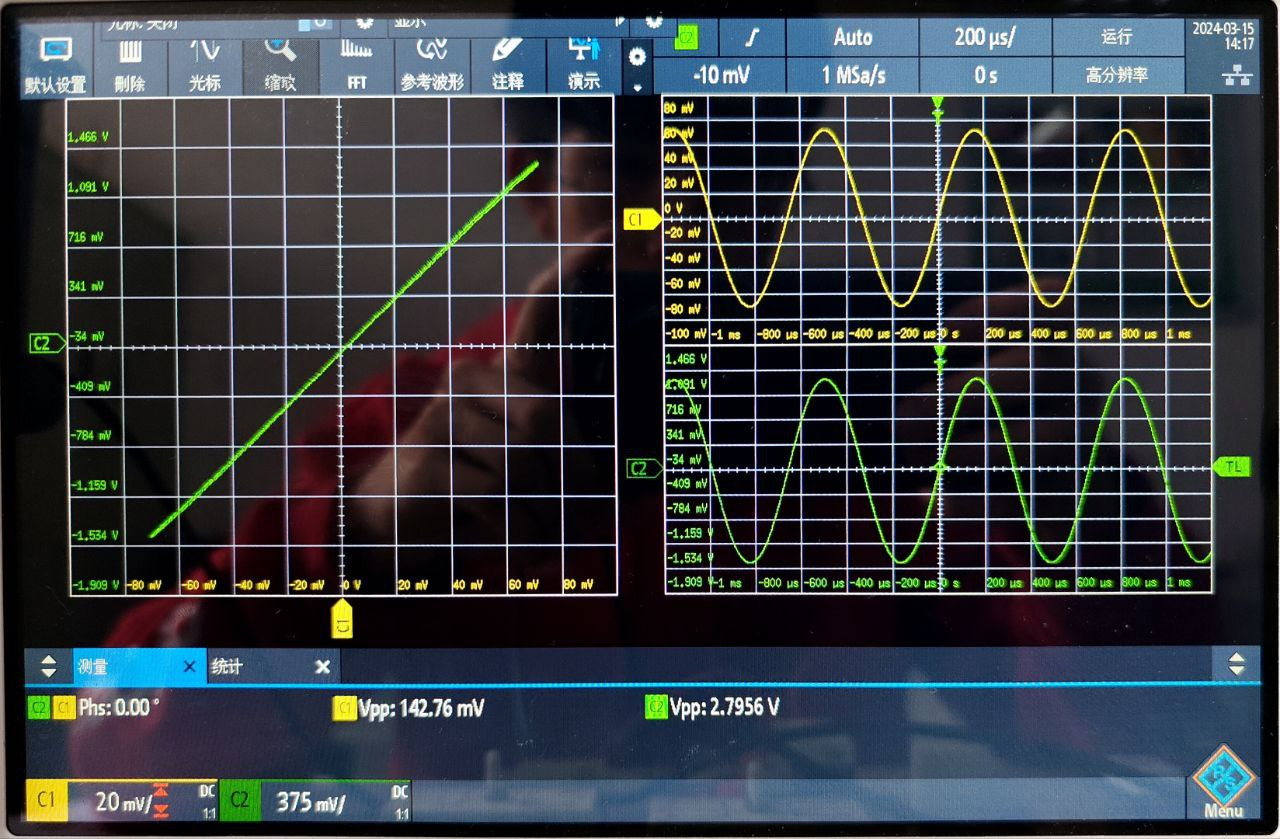
\includegraphics[width=0.6\textwidth]{resonance.jpg}
\caption{共振时示波器图形}\label{fig:resonance}
\end{figure}
\\测量得到的共振频率为$f_0=1.558kHz$。使用公式计算为$f_0=\frac{1}{2\pi\sqrt{LC}}=1.592kHz$。两者相差不大,说明实验测量结果较为准确。
\\测量值稍小于理论值可能原因是电路中寄生的电容和电感所致。
\subsubsection{在谐振频率下测量Q值}
\begin{enumerate}
    \item 调整电路交换电阻电容位置
    \item 使用示波器测量电容两侧电压峰峰值和输入电压峰峰值
\end{enumerate}
测量得到$V_{pp,in},V_{pp,C}$,计算得到电路的品质因数$Q=\frac{V_{pp,C}}{V_{pp,in}}=0.100$
\subsubsection{测量不同频率下增益和相位差}
\begin{enumerate}
    \item 改变电路结构,交换电阻和电容位置,将示波器接入电阻两端;
    \item 调整信号发生器频率,测量不同频率下两信号电压幅值和相位差
    \item 作图并分析
\end{enumerate}
根据上述实验得到数据进行绘图,并使用公式
\begin{equation}
    A = \frac{1}{\sqrt{1 + Q^2(\frac{\omega_0}{\omega} - \frac{\omega}{\omega_0})^2}}, \quad
    \phi = \arctan\left[Q\left(\frac{\omega_0}{\omega} - \frac{\omega}{\omega_0}\right)\right]
\end{equation}
计算得到的理论幅值和相位差进行对比。如图\ref{fig:gain}和图\ref{fig:phase}所示。
理论值计算中使用的参数为:
\begin{equation}
    f_0=\frac{1}{2\pi\sqrt{LC}}=1.558kHz\ ;\ Q = \frac{1}{R}\sqrt{\frac{L}{C}}=0.0.996
\end{equation}
\begin{figure}[htbp]
        \centering
    \begin{minipage}[t]{0.48\textwidth}
        \centering
        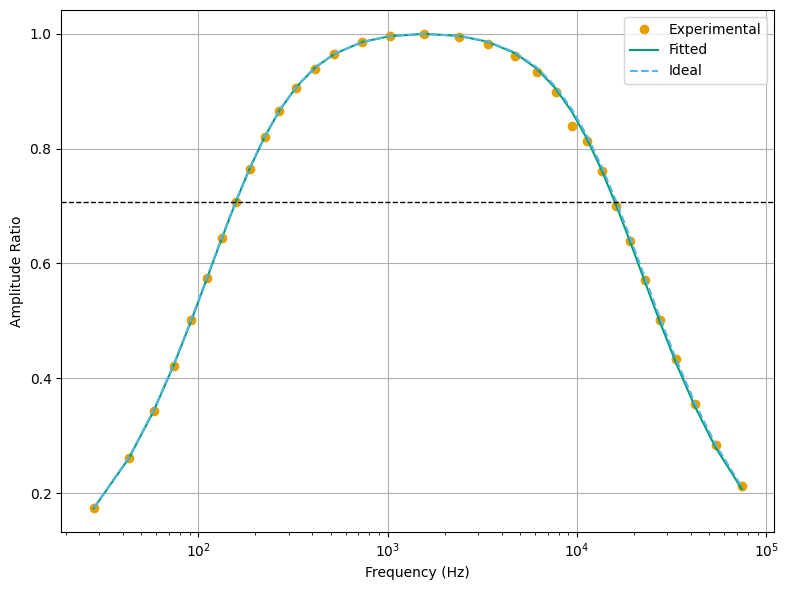
\includegraphics[width=\textwidth]{gain.png}
        \caption{增益-频率特性曲线}\label{fig:gain}
        \label{fig:gain}
    \end{minipage}
    \begin{minipage}[t]{0.48\textwidth}
        \centering
        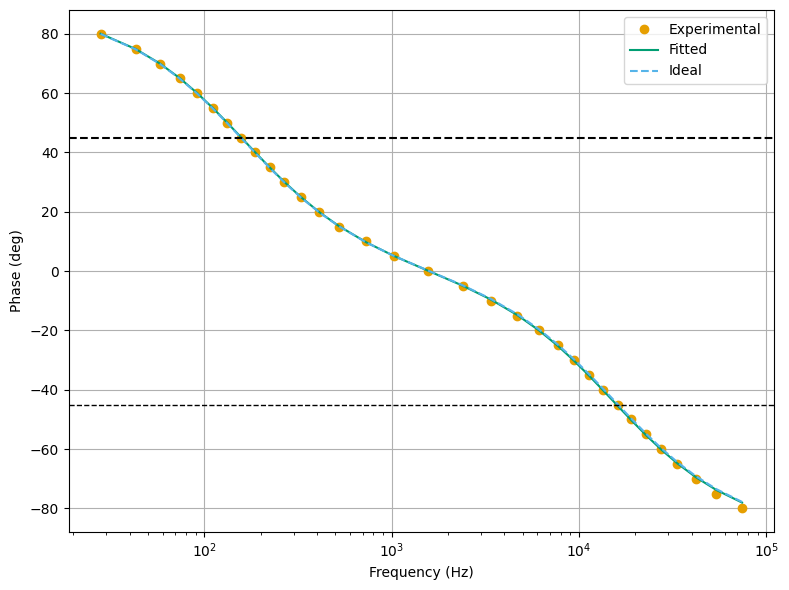
\includegraphics[width=\textwidth]{phase.png}
        \caption{相位差-频率特性曲线}\label{fig:phase}
        \label{fig:phase}
    \end{minipage}
\end{figure}
\\
图中黑色虚线为
\\
另外,我们还使用回归计算方法得到电路的品质因数和谐振频率:
$$ f_0=1580.42 Hz\ ;\ Q =0.101$$
增益-频率特性曲线和相位差-频率特性曲线与理论值符合较好,说明实验结果较为准确。其中在$10^4 Hz$附近有一个数据点为离群值,可能是由于测量失误所致。
\section{分析与讨论}
\subsection{实验结果分析}
\begin{enumerate}
    \item 通过实验第一部分测量得到的共振频率与理论值相差不大,实验测量结果较为准确。
    \begin{enumerate}
        \item 实验测量值为$f_0=1.558kHz$,理论值为$f_0=1.592kHz$。
        \item 实验值略小于理论值,可能是电路中寄生的电容和电感所致。
        \item 不排除由于测量中无法准确判断相位差零点的影响。
    \end{enumerate} 
    \item 通过实验测量得到的品质因数与理论值相差不大,实验测量结果较为准确。
    \begin{enumerate}
        \item 实验测量值为$Q=0.10$,理论值为$Q=0.996$。
        \item 测量值略大于理论值,这是在实验误差之内的结果。
    \end{enumerate}
    \item 通过实验测量得到的增益-频率特性曲线和相位差-频率特性曲线与理论值符合较好,说明实验结果较为准确。
    \begin{enumerate}
        \item 由理论值计算得到的增益-频率特性曲线和相位差-频率特性曲线与实验测量值拟合得到符合较好,在全频段均无较大差异。
        \item 实验数据点与理论以及拟合曲线有一到两个数据点的偏离,可能是由于测量失误所致。
        \item 拟合结果在特征频率上相较第一部分结果更接近理论值,但依然小于理论值进一步说明了电路中寄生的电容和电感所致。
        \item 得到的拟合曲线在半对数坐标轴上符合理论预测的特征:
        \begin{enumerate}
            \item 增益在特征频率上有一个单峰且关于特征频率对称;
            \item 相位差在关于频率单调且在特征频率上有一个零点,且为奇函数。
        \end{enumerate}
        \item 在频率最高的两个数据点处有一定便宜,这可能是由于电路元件的非线性以及测量仪器的频率响应特性所致。
    \end{enumerate}
\end{enumerate}
\section{附录}
\subsection{原始数据}

\begin{table}[htbp]
\centering
\begin{tabular}{|l|l|l|l|l|l|l|l|l|}
元件&特征值&单位&电阻值&单位&谐振频率&U\_c&U\_0&Q\\
电感&10&mH&14.25&Ohm&1558hz&0.96&9.31&0.10\\
电阻&1,000&Ohm&990&Ohm&&&&\\
电容&1&uf&N/A&N/A&&&&\\
\end{tabular}
\end{table}

\begin{table}[htbp]
\centering
\begin{tabular}{|l|l|l|l|l|}
f&U\_r&U\_0&A&phi\\
28&1.71&9.97&0.17&-80\\
43&2.57&9.96&0.26&-75\\
58&3.35&9.93&0.34&-70\\
74&4.12&9.90&0.42&-65\\
92&4.88&9.86&0.49&-60\\
111&5.56&9.82&0.57&-55\\
133&6.21&9.79&0.63&-50\\
158&6.80&9.75&0.70&-45\\
187&7.33&9.72&0.75&-40\\
224&7.82&9.67&0.81&-35\\
268&8.22&9.64&0.85&-30\\
328&8.58&9.61&0.89&-25\\
411&8.88&9.59&0.93&-20\\
523&9.09&9.56&0.95&-15\\
734&9.24&9.50&0.97&-10\\
1,028&9.19&9.36&0.98&-5\\
1,558&9.17&9.30&0.99&0\\
2,390&9.13&9.32&0.98&5\\
3,370&9.04&9.33&0.97&10\\
4,690&8.86&9.35&0.95&15\\
6,120&8.63&9.37&0.92&20\\
7,720&8.32&9.40&0.89&25\\
9,400&7.80&9.43&0.83&30\\
11,290&7.58&9.46&0.80&35\\
13,490&7.12&9.50&0.75&40\\
16,137&6.58&9.54&0.69&45\\
19,040&6.04&9.58&0.63&50\\
22,880&5.41&9.62&0.56&55\\
27,480&4.77&9.66&0.49&60\\
33,480&4.14&9.69&0.43&65\\
41,980&3.41&9.72&0.35&70\\
53,980&2.74&9.77&0.28&75\\
74,080&2.04&9.79&0.21&80\\
\end{tabular}
\end{table}
\newpage
\subsection{代码}
\begin{python}
import numpy as np
import pandas as pd
import matplotlib.pyplot as plt
from scipy.optimize import curve_fit

df = pd.read_excel('data.xlsx', sheet_name='freqA')
# 定义电路数据
R = 990
L = 0.01
C = 1e-6
R_L = 14.25

# 读取实验数据
freq = pd.to_numeric(df['f'], errors='coerce')
U_r = pd.to_numeric(df['U_r'], errors='coerce')
U_0 = pd.to_numeric(df['U_0'], errors='coerce')
phi_exp = -pd.to_numeric(df['phi'], errors='coerce')
f0_exp = 1558
Q_exp = 0.103115

# 计算幅值比A和修正后的幅值比A'
A = U_r / U_0
A_exp = (R + R_L) / R * A



# 定义理论值计算函数
def A_theory(f, f0, Q):
    return 1 / np.sqrt(1 + Q**2 * (f0/f - f/f0)**2)

def phi_theory(f, f0, Q):
    return np.arctan(Q * (f0/f - f/f0)) * 180 / np.pi

# 计算理想值
w0 = 1 / np.sqrt(L * C)
Q = 1 / (R + R_L) * np.sqrt(L / C)
w = 2 * np.pi * freq
A_ideal = 1 / np.sqrt(1 + Q**2 * (w0/w - w/w0)**2)
phi_ideal = np.arctan(Q * (w0/w - w/w0)) * 180 / np.pi

# 定义回归函数
def A_fit(f, f0, Q):
    return A_theory(f, f0, Q)

def phi_fit(f, f0, Q):
    return phi_theory(f, f0, Q)

# 进行数据回归
popt_A, _ = curve_fit(A_fit, freq, A_exp)
popt_phi, _ = curve_fit(phi_fit, freq, phi_exp)

# 计算回归曲线
A_fit_val = A_fit(freq, *popt_A)
phi_fit_val = phi_fit(freq, *popt_phi)


# 定义配色方案
colors = {'exp': '#E69F00', 'theory': '#56B4E9', 'fit': '#009E73', 'bw': '#D55E00'}

# 绘制幅频响应曲线
plt.figure(figsize=(8, 6))
plt.semilogx(freq, A_exp, 'o', label='Experimental', color=colors['exp'])
plt.semilogx(freq, A_fit_val, '-', label='Fitted', color=colors['fit'])
plt.semilogx(freq, A_ideal, '--', label='Ideal', color=colors['theory'])
plt.xscale('log')
plt.xlabel('Frequency (Hz)')
plt.ylabel('Amplitude Ratio')
plt.legend()
plt.grid(True)

# 绘制带宽横竖线
f1, f2 = popt_A[0] / (1 + 1/(2*popt_A[1])), popt_A[0] * (1 + 1/(2*popt_A[1]))
plt.axvline(f1, color='k', linestyle='--', label='Bandwidth', lw=1)
plt.axvline(f2, color='k', linestyle='--', lw=1)
plt.axhline(max(A_fit_val)/np.sqrt(2), color='k', linestyle='--', lw=1)
plt.tight_layout()
plt.show()

# 绘制相频响应曲线
plt.figure(figsize=(8, 6))
plt.semilogx(freq, phi_exp, 'o', label='Experimental', color=colors['exp'])
plt.semilogx(freq, phi_fit_val, '-', label='Fitted', color=colors['fit'])
plt.semilogx(freq, phi_ideal, '--', label='Ideal', color=colors['theory'])
plt.xscale('log')
plt.xlabel('Frequency (Hz)')
plt.ylabel('Phase (deg)')
plt.legend()
plt.grid(True)

# 绘制带宽横竖线
plt.axvline(f1, color='k', linestyle='--', lw=1)
plt.axvline(f2, color='k', linestyle='--', lw=1)
plt.axhline(-45, color='k', linestyle='--', lw=1)
plt.axhline(45, color='k', linestyle='--')

plt.tight_layout()
plt.show()


f0_fit, Q_fit = popt_A
print(f"拟合得到的谐振频率: {-f0_fit:.2f} Hz, 品质因数: {Q_fit:.3f}")
\end{python}
\end{document}
